% =============================================================================================
% Multimedia Retrieval assignment: technical report.
% Images used by the report: the folders Images/ and figures/step1_smooth/ next to this file.
% =============================================================================================
\documentclass[10pt,a4paper]{article}

\usepackage[T1]{fontenc}
\usepackage[utf8]{inputenc}
\usepackage{lmodern}
\usepackage[a4paper,top=2.0cm,bottom=2.0cm,left=2.2cm,right=2.2cm]{geometry}
\usepackage{microtype}

% mathematics
\usepackage{amsmath,amssymb}

% figures and tables
\usepackage{graphicx}
\usepackage{adjustbox}
\usepackage{booktabs}
\usepackage{array}
\usepackage[font=small,labelfont=bf,skip=3pt]{caption}
\usepackage{subcaption}
\usepackage{xcolor}
\usepackage{tikz}
\usetikzlibrary{arrows.meta,positioning}
\usepackage{enumitem}
\usepackage{url}

% compact spacing
\setlength{\parindent}{0pt}
\setlength{\parskip}{3.5pt plus 1pt}
\linespread{1.0}
\usepackage{titlesec}
\titlespacing*{\section}{0pt}{12pt plus 2pt minus 2pt}{5pt plus 1pt}
\titlespacing*{\subsection}{0pt}{9pt plus 2pt minus 2pt}{3pt plus 1pt}
\titlespacing*{\subsubsection}{0pt}{7pt plus 2pt minus 1pt}{2pt plus 1pt}
\titleformat{\section}{\large\bfseries}{\thesection}{0.6em}{}
\titleformat{\subsection}{\normalsize\bfseries}{\thesubsection}{0.6em}{}
\titleformat{\subsubsection}{\normalsize\bfseries\itshape}{\thesubsubsection}{0.6em}{}
\setlength{\textfloatsep}{9pt plus 2pt minus 2pt}
\setlength{\floatsep}{7pt plus 2pt minus 2pt}
\setlength{\intextsep}{7pt plus 2pt minus 2pt}
\renewcommand{\arraystretch}{1.08}
\setlist{nosep,leftmargin=1.4em}

% numbering: tables and figures are numbered per section (Table 2.3, Figure 1.4, ...)
\setcounter{secnumdepth}{3}
\usepackage{chngcntr}
\counterwithin{table}{section}
\counterwithin{figure}{section}
\counterwithin{equation}{section}

% figures are found in these folders
\graphicspath{{Images/}{figures/step1_smooth/}}

% shortcuts used in the text
\newcommand{\R}{\mathbb{R}}
\newcommand{\card}[1]{\lvert #1\rvert}

% hyperref last
\usepackage[hidelinks,pdfusetitle]{hyperref}

\title{Multimedia Retrieval -- Practical Assignment}
\author{Maria Podbylska (4339304) \and Bharath Kumar Sokke Prabhu (8874476)}
\date{}

\begin{document}
\pagestyle{plain}

% ---------------------------------------------------------------------------------------------
% Title page
% ---------------------------------------------------------------------------------------------
\begin{titlepage}
\centering
\vspace*{1.5cm}
{\normalsize Utrecht University\par}
\vspace{3pt}
{\normalsize Multimedia Retrieval\par}
\vspace{\stretch{0.6}}
\rule{0.85\linewidth}{0.6pt}\par
\vspace{0.8cm}
{\fontsize{30}{38}\selectfont\bfseries Practical Assignment\\ Technical Report\par}
\vspace{1.2cm}
{\LARGE Maria Podbylska (4339304)\par}
\vspace{8pt}
{\LARGE Bharath Kumar Sokke Prabhu (8874476)\par}
\vspace{0.9cm}
\rule{0.85\linewidth}{0.6pt}\par
\vspace{\stretch{2}}
{\normalsize Lecturer: prof.\ dr.\ Alex Telea\par}
\vspace{4pt}
{\normalsize \ifnum\day<10 0\fi\the\day.\ifnum\month<10 0\fi\the\month.\the\year\par}
\vspace*{1cm}
\end{titlepage}

\section*{Recent Changes}
\textbf{General:} changes to the whole report.
\begin{itemize}
  \item \textbf{Format:} the report is now written in LaTeX. The layout was made more compact.
  \item \textbf{Report structure:} a title page, a table of contents and numbered sections were added. Figures, tables and
        equations are now numbered and referenced in the text.
  \item \textbf{References:} the references are numbered in the order in which they are cited and are listed on a separate
        last page.
  \item \textbf{Introduction:} sections about the purpose and the structure of the report were added (Section~\ref{sec:intro}).
  \item \textbf{Mathematical notation:} formal definitions of the mesh, the face type, the axis-aligned bounding box, the
        face orientation and the signed volume were added, together with a table of all symbols used in the report (Section~\ref{sec:notation}).
        The former Section~1.2 is merged into this section.
  \item \textbf{Software and tools:} a table with the exact versions and sources of all tools was added
        (Section~\ref{sec:tools}), and every tool now has a reference. Version numbers were removed from the running text.
\end{itemize}
\textbf{Step 1:} the first version was edited.
\begin{itemize}
  \item \textbf{Text:} the text was revised to be more concise.
  \item \textbf{Face type:} the face type is now measured: all 2,483 shapes consist of triangles only
        (Section~\ref{sec:loading}). Table~\ref{tab:six} now also lists the file and the face type of each shape.
  \item \textbf{Shading of the Hand shape:} the coloured patches in the former Figure~4 were investigated. The patches are an
        artifact of flat shading. All shapes are now rendered with smooth shading (Section~\ref{sec:results1},
        Figure~\ref{fig:handshading}).
  \item \textbf{Figures:} each figure shows the shaded and wireframe views as subfigures (a) and (b) in the same order. The
        captions name the file of the shape and describe what is shown.
\end{itemize}
\textbf{Step 2:} the first version was added.
\clearpage

{\small\tableofcontents}
\clearpage

\section{Introduction}\label{sec:intro}

\subsection{Purpose and Scope}
This report documents the design and implementation of a content-based 3D shape retrieval system, developed for the Multimedia
Retrieval course at Utrecht University~[1]. Given a query shape, the system returns the shapes of a database that are most
similar to it. The database contains 2,483 shapes in 69 classes, stored as Wavefront OBJ files~[2].

\subsection{Structure of the Report}
Section~\ref{sec:step1} describes how the shapes are read from disk and visualized, and Section~\ref{sec:step2} describes
the analysis and preprocessing of the shape database. The rest of this section introduces the mathematical notation
(Section~\ref{sec:notation}) and the software that was used (Section~\ref{sec:tools}).

\subsection{Mathematical Notation}\label{sec:notation}

\paragraph{Shapes.}
A shape is represented by a mesh $M=(V,F)$, where
\begin{equation}
  V=\{v_i\},\quad 1\le i\le N_V,\quad v_i=(x_i,y_i,z_i)\in\R^3
  \label{eq:vertices}
\end{equation}
is the set of vertices and
\begin{equation}
  F=\{f_j\},\quad 1\le j\le N_F,\quad f_j=(v_j^1,\dots,v_j^{k_j}),\quad 1\le v_j^l\le N_V
  \label{eq:faces}
\end{equation}
is the set of faces. A face is a tuple of $k_j=\card{f_j}\ge 3$ vertex indices. A face with $k_j=3$ is a triangle,
$f_j=(v_j^1,v_j^2,v_j^3)$, and a face with $k_j=4$ is a quad. The face type of a mesh is
$\tau(M)=\textit{triangles}$ if $k_j=3$ for all $j$, $\tau(M)=\textit{quads}$ if $k_j=4$ for all $j$, and
$\tau(M)=\textit{mixed}$ otherwise. The face type is not assumed but measured for every shape (Section~\ref{sec:step2}).
The database also provides a class label $c(M)\in\mathcal{C}$, $\card{\mathcal{C}}=69$, for each shape through its folder
structure. For example, shapes stored in the Bicycle, Bird, or House folders belong to those respective classes. The class labels are
used later to evaluate the retrieval results.

\paragraph{Axis-Aligned Bounding Box.}
The axis-aligned bounding box (AABB) of $M$ is the smallest box with faces parallel to the coordinate planes that contains all
vertices of $M$:
\begin{gather}
  B(M)=[x_{\min},x_{\max}]\times[y_{\min},y_{\max}]\times[z_{\min},z_{\max}],\label{eq:aabb}\\
  x_{\min}=\min_{1\le i\le N_V}x_i,\quad y_{\min}=\min_{1\le i\le N_V}y_i,\quad z_{\min}=\min_{1\le i\le N_V}z_i,\notag\\
  x_{\max}=\max_{1\le i\le N_V}x_i,\quad y_{\max}=\max_{1\le i\le N_V}y_i,\quad z_{\max}=\max_{1\le i\le N_V}z_i .\notag
\end{gather}
Its diagonal is $d(M)=\lVert(x_{\max}-x_{\min},\,y_{\max}-y_{\min},\,z_{\max}-z_{\min})\rVert$.

\paragraph{Orientation.}
The directed edges of a face $f_j$ are $(v_j^l,v_j^{l+1})$, with $l$ taken modulo $k_j$. Two faces that share an edge are
consistently oriented if they traverse the shared edge in opposite directions; a mesh in which this holds for all shared edges
is consistently oriented. The unit normal of a triangle $f_j$ is
\begin{equation}
  n_j=\frac{(v_j^2-v_j^1)\times(v_j^3-v_j^1)}{\lVert(v_j^2-v_j^1)\times(v_j^3-v_j^1)\rVert}.
  \label{eq:normal}
\end{equation}
For a triangle mesh, the signed volume is
\begin{equation}
  \mathrm{Vol}(M)=\frac16\sum_{j=1}^{N_F} v_j^1\cdot\big(v_j^2\times v_j^3\big).
  \label{eq:signedvolume}
\end{equation}
For a closed, consistently oriented mesh, $\mathrm{Vol}(M)>0$ if the normals point outwards and $\mathrm{Vol}(M)<0$ if they
point inwards.

\paragraph{Overview.}
Table~\ref{tab:notation} lists all symbols used in the report, together with the section in which they are defined.

\begin{table}[htbp]\centering\small
\begin{tabular}{@{}p{0.30\linewidth}p{0.55\linewidth}l@{}}\toprule
Symbol & Meaning & Section\\\midrule
$M=(V,F)$, $N_V$, $N_F$ & mesh, number of vertices, number of faces & \ref{sec:notation}\\
$v_i=(x_i,y_i,z_i)$, $f_j$, $k_j$ & vertex, face, number of corners of a face & \ref{sec:notation}\\
$\tau(M)$, $c(M)$, $\mathcal{C}$ & face type, class label, set of classes & \ref{sec:notation}\\
$B(M)$, $d(M)$ & axis-aligned bounding box and its diagonal & \ref{sec:notation}\\
$n_j$ & unit normal of triangle $f_j$ & \ref{sec:notation}\\
$\mathrm{Vol}(M)$ & signed volume & \ref{sec:notation}\\
$\bar v$ & barycenter of the shape & ?\\
$\lambda_1\ge\lambda_2\ge\lambda_3$, $e_1,e_2,e_3$ & eigenvalues and eigenvectors of the vertex covariance matrix & ?\\
\bottomrule\end{tabular}
\caption{Notation used in this report.}\label{tab:notation}
\end{table}

\subsection{Software and Tools}\label{sec:tools}
The system is implemented in Python. All libraries were installed from the Python Package Index (PyPI) with \texttt{pip} into a
virtual environment, on Windows~11. Table~\ref{tab:tools} lists the exact versions and the source of every tool.

\begin{table}[htbp]\centering\small
\begin{tabular}{@{}llp{0.33\linewidth}l@{}}\toprule
Tool & Version & Use & Source\\\midrule
Python~[3]     & 3.12.10 & programming language & \url{https://www.python.org}\\
trimesh~[4]    & 5.1.0   & loading OBJ files, mesh processing & \url{https://trimesh.org}\\
NumPy~[5]      & 2.5.3   & numerical arrays & \url{https://numpy.org}\\
pandas~[6]     & 3.0.6   & tables of per-shape statistics & \url{https://pandas.pydata.org}\\
Plotly~[7]     & 7.1.0   & interactive 3D viewer & \url{https://plotly.com/python}\\
Kaleido~[8]    & 1.4.0   & export of rendered views as images & \url{https://github.com/plotly/Kaleido}\\
Open3D~[9]     & 0.20.0  & standalone viewer, mesh resampling & \url{https://www.open3d.org}\\
Matplotlib~[10] & 3.11.2 & histograms and plots & \url{https://matplotlib.org}\\
Tectonic~[11]  & 0.17.0  & compiling this report (LaTeX) & \url{https://tectonic-typesetting.github.io}\\
\bottomrule\end{tabular}
\caption{Software used, with exact versions and sources.}\label{tab:tools}
\end{table}

\section{Step 1: Reading and Viewing 3D Shape Data}\label{sec:step1}

\subsection{Aim}
The goal of this step is an application that reads the 3D shapes of the database and displays them. A mesh is shown with shaded
rendering, optionally with its edges drawn, and the user can rotate, zoom and pan the view.

The application is also a way to get to know the structure and variety of the database before any further processing. It was
therefore tested on several different shapes rather than on a single example. Figure~\ref{fig:pipeline1} shows the pipeline.

\begin{figure}[htbp]\centering
\small OBJ file $\rightarrow$ Mesh loader $\rightarrow$ Vertices and faces $\rightarrow$ 3D viewer $\rightarrow$ Interactive visualization
\caption{Pipeline of the reading and viewing application.}\label{fig:pipeline1}
\end{figure}

\subsection{Data Format}
The database stores the shapes in Wavefront OBJ format. OBJ is a text-based format in which the geometry can be described using
vertex and face definitions.

Figure~\ref{fig:obj} shows an excerpt of such a file.

\begin{figure}[htbp]\centering

\includegraphics[width=0.75\linewidth]{OBJ_excerpt.png}
\caption{Excerpt of an OBJ file with vertex (\texttt{v}) and face (\texttt{f}) lines.}\label{fig:obj}
\end{figure}

The v lines contain the coordinates $(x_i,y_i,z_i)$ of the vertices $v_i$, while the f lines specify which vertices form each
face $f_j$.

The database files consist mainly of vertex and face lines. Texture coordinates, normals and materials are not used by the
viewer.

\subsection{Design and Implementation}\label{sec:design1}
The application is written in Python and uses trimesh~[4] for loading the meshes and Plotly~[7] for the interactive view.
The trimesh library was chosen because it reads OBJ files directly and gives access to the vertices and faces as NumPy arrays.
In addition, a standalone viewer based on Open3D~[9] was written for fast exploration, and Kaleido~[8] was used to export
rendered views as images.

The surface is displayed with Plotly's \texttt{Mesh3d}. Shading makes the three-dimensional structure easier to see. Smooth
shading is used, in which the colour is interpolated from normals averaged at the vertices, because flat shading of dense meshes
produces visual artifacts (Section~\ref{sec:results1}). The optional wireframe is drawn from the edges of the faces.

The viewer supports the following interaction:
\begin{itemize}
  \item rotation by dragging the model;
  \item zooming with the mouse wheel;
  \item panning with the mouse and keyboard;
  \item switching the wireframe on and off.
\end{itemize}

\subsection{Mesh Loading}\label{sec:loading}
All shapes are loaded by one function that reads an OBJ file with trimesh and returns the mesh $M=(V,F)$ as NumPy arrays.
Two loading options are set explicitly. First, the result is forced into a triangle mesh, so that faces with more than three
vertices would be split into triangles that the renderer can display. Second, the automatic processing of trimesh is switched
off, so that the data is kept exactly as stored in the file. Otherwise duplicate vertices would be merged and degenerate faces
removed without notice, which would distort the statistics of Section~\ref{sec:step2}. The same function is used for every
shape in this report.

Because triangulation during loading would hide the original face type $\tau(M)$, the face type is determined separately, by
reading the \texttt{f} lines of the OBJ files directly (Section~\ref{sec:step2}). All 2,483 shapes consist of triangles only,
so the triangulation never changes a mesh.

\subsection{Results}\label{sec:results1}
The loader and the viewer were tested with one shape from each of six classes: Bicycle, Bird, Chess, Hand, House and Tree.
Table~\ref{tab:six} lists their vertex and face counts.

\begin{table}[htbp]\centering\small
\begin{tabular}{@{}llrrl@{}}
\toprule
Class & File & $N_V$ & $N_F$ & $\tau(M)$ \\
\midrule
Bicycle & D00016 & 2,769 & 5,049 & triangles \\
Bird & D00089 & 233 & 462 & triangles \\
Chess & D01017 & 380 & 756 & triangles \\
Hand & D01006 & 7,929 & 15,855 & triangles \\
House & D00001 & 46,622 & 90,161 & triangles \\
Tree & D00096 & 54,223 & 36,512 & triangles \\
\bottomrule
\end{tabular}
\caption{Number of vertices $N_V$, number of faces $N_F$ and face type $\tau(M)$ of the six shapes used to test the viewer.}
\label{tab:six}
\end{table}

The shapes were chosen because their geometry differs: the Bicycle has many thin mechanical parts, the Bird and the Hand are
organic shapes, the House has large flat surfaces, and the Tree branches strongly. Their sizes range from 233 to 54,223 vertices.

Figures~\ref{fig:bicycle}--\ref{fig:tree} show each shape shaded and with the wireframe overlay. All six shapes could be
rotated, zoomed and panned without problems.

The loader was also run on the whole database. All 2,483 OBJ files in 69 classes were loaded without exceptions, and none of
the meshes was empty. This only shows that the files can be parsed, not that the meshes are free of geometric problems; these
are analysed in Section~\ref{sec:step2}.

% \reportfig{shape}{label}{caption}   (images are in the folder figures/step1_smooth/)
\newcommand{\reportfig}[3]{%
\begin{figure}[htbp]\centering
\begin{subfigure}{0.48\linewidth}\centering\includegraphics[width=\linewidth]{#1_shaded.png}\caption{shaded}\end{subfigure}\hfill
\begin{subfigure}{0.48\linewidth}\centering\includegraphics[width=\linewidth]{#1_wireframe.png}\caption{shaded with wireframe}\end{subfigure}
\caption{#3}\label{#2}
\end{figure}}
\reportfig{Bicycle}{fig:bicycle}{Bicycle (D00016), a mechanical shape with many thin parts: (a) smooth shading, (b) with the wireframe drawn on top.}
\reportfig{Bird}{fig:bird}{Bird (D00089), the smallest of the six test shapes (233 vertices): (a) smooth shading, (b) with the wireframe drawn on top.}
\reportfig{Chess}{fig:chess}{Chess piece (D01017), a small rotationally symmetric shape: (a) smooth shading, (b) with the wireframe drawn on top.}
\reportfig{Hand}{fig:hand}{Hand (D01006), an organic shape with a dense, irregular mesh: (a) smooth shading, (b) with the wireframe drawn on top.}
\reportfig{House}{fig:house}{House (D00001), an architectural shape with large flat surfaces: (a) smooth shading, (b) with the wireframe drawn on top.}
\reportfig{Tree}{fig:tree}{Tree (D00096), the largest of the six test shapes (54,223 vertices), with a strongly branching structure: (a) smooth shading, (b) with the wireframe drawn on top.}

\paragraph{Shading of the Hand Shape.}
With flat shading, in which every triangle receives one colour computed from its normal $n_j$, the Hand shows irregular dark
patches (Figure~\ref{fig:handshading}a). Such patches are typical for inconsistently oriented faces, whose normals point to the
inside of the surface, so the orientation of the Hand mesh was checked. The mesh is consistently oriented: none of its 23,782 edges is
traversed in the same direction by its two faces, and its signed volume (Eq.~\eqref{eq:signedvolume}) is positive, which means that the normals point
outwards. As an additional test, the orientation of every face was reversed; the flat-shaded image remains the same
(Figure~\ref{fig:handshading}b), so the patches do not depend on the face orientation. They are an artifact of flat shading
in the renderer for dense meshes with many small triangles. With smooth shading the surface is displayed correctly
(Figure~\ref{fig:handshading}c), and smooth shading is therefore used for all figures in this report.

Inconsistent orientation does occur elsewhere in the database: 693 of the 2,483 shapes (28\,\%), including the Bicycle and
the House of Table~\ref{tab:six}, contain inconsistently oriented faces. These will be reoriented during preprocessing
(Section~\ref{sec:step2}).

\begin{figure}[htbp]\centering
\begin{subfigure}{0.32\linewidth}\centering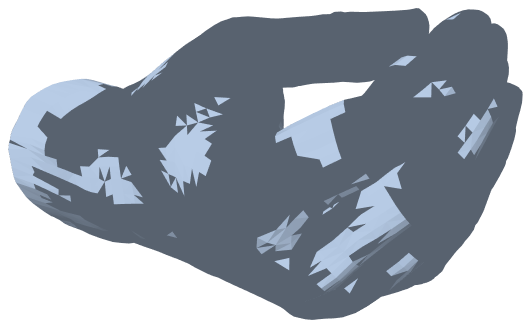
\includegraphics[width=\linewidth]{hand_flat_crop.png}\caption{flat shading}\end{subfigure}\hfill
\begin{subfigure}{0.32\linewidth}\centering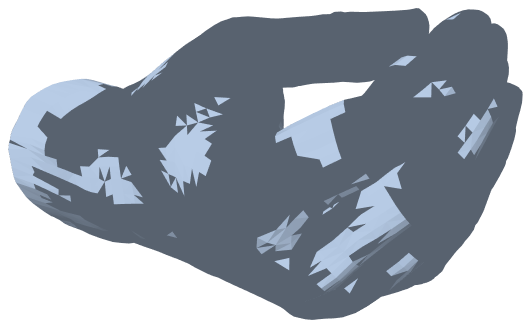
\includegraphics[width=\linewidth]{hand_flat_reversed_crop.png}\caption{flat, all faces reversed}\end{subfigure}\hfill
\begin{subfigure}{0.32\linewidth}\centering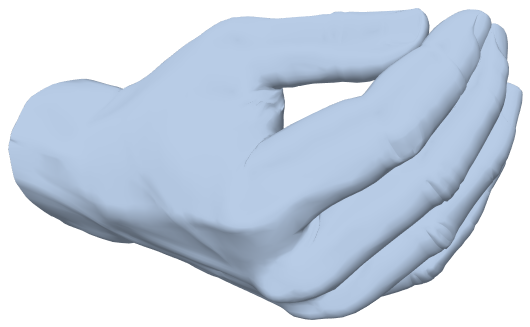
\includegraphics[width=\linewidth]{hand_smooth_crop.png}\caption{smooth shading}\end{subfigure}
\caption{The Hand shape (D01006): (a) flat shading shows dark patches; (b) the patches stay the same when all faces are reversed, so they are not caused by the face orientation; (c) smooth shading shows the surface correctly.}\label{fig:handshading}
\end{figure}

\subsection{Discussion}
The application reads the OBJ files of the database, converts them into the mesh representation $M=(V,F)$, and displays them
interactively. The same loading function is used for the viewer and for the test on the whole database, so both rely on
exactly the same data.

Testing with shapes of very different size and structure was useful, because the database varies strongly in mesh resolution
and complexity: the six test shapes alone range from 233 to 54,223 vertices. A single simple model would not have revealed
problems such as the shading artifacts of the Hand, which only appear for dense meshes with many small triangles.

The viewer works on triangulated data, so the original face type cannot be read from the loaded mesh. For the analysis of the
database it is therefore determined from the OBJ files directly (Section~\ref{sec:loading}). In the same way, a successful load
says nothing about the quality of a mesh. Problems such as inconsistent face orientation, duplicate vertices or degenerate
faces have to be detected separately, which is done in Section~\ref{sec:step2}.

\subsection{Conclusion}
The application loads OBJ meshes with trimesh and displays them interactively with Plotly. It supports shaded rendering with an
optional wireframe, together with rotation, zooming and panning. Smooth shading is used, because flat shading produced
misleading artifacts on dense meshes.

The viewer was tested on six shapes from different classes, from small meshes such as the Bird and the Chess piece to much
larger meshes such as the House and the Tree, and the loader reads all 2,483 shapes of the database without errors. The
application is used to inspect the shapes during the preprocessing described in Section~\ref{sec:step2}.

\section{Step 2: Preprocessing and Cleaning}\label{sec:step2}

\clearpage
\section*{References}
\addcontentsline{toc}{section}{References}
\begin{description}[leftmargin=2.2em,labelwidth=2em,style=sameline]\sloppy
\item[{[1]}] A. C. Telea, Multimedia Retrieval -- Assignment, Utrecht University. Available:
  \url{https://webspace.science.uu.nl/~telea001/MR/Assignment}.
\item[{[2]}] MaxRee94, ShapeDatabase\_INFOMR, GitHub repository. Available: \url{https://github.com/MaxRee94/ShapeDatabase_INFOMR}.
  Shape database used for this project.
\item[{[3]}] Python Software Foundation, Python Language Reference, version 3.12.10. Available: \url{https://www.python.org}.
\item[{[4]}] M. Dawson-Haggerty et al., Trimesh: Python library for loading and processing triangular meshes, version 5.1.0.
  Available: \url{https://trimesh.org}. Used for loading and handling the OBJ mesh data.
\item[{[5]}] C. R. Harris et al., Array programming with NumPy, \emph{Nature}, 585:357--362, 2020. NumPy version 2.5.3. Available:
  \url{https://numpy.org}.
\item[{[6]}] W. McKinney, Data structures for statistical computing in Python, \emph{Proceedings of the 9th Python in Science
  Conference}, 56--61, 2010. pandas version 3.0.6. Available: \url{https://pandas.pydata.org}.
\item[{[7]}] Plotly Technologies Inc., Plotly Python Graphing Library, version 7.1.0. Available: \url{https://plotly.com/python/}.
  Used for interactive 3D mesh visualization.
\item[{[8]}] Plotly Technologies Inc., Kaleido, version 1.4.0. Available: \url{https://github.com/plotly/Kaleido}. Used to export
  images of the rendered shapes for this report.
\item[{[9]}] Open3D Development Team, Open3D, version 0.20.0. Available: \url{https://www.open3d.org}. Used for the standalone
  mesh viewer.
\item[{[10]}] J. D. Hunter, Matplotlib: A 2D graphics environment, \emph{Computing in Science \& Engineering}, 9(3):90--95,
  2007. Matplotlib version 3.11.2. Available: \url{https://matplotlib.org}.
\item[{[11]}] The Tectonic Project, Tectonic: a modernized, complete, self-contained TeX/LaTeX engine, version 0.17.0. Available:
  \url{https://tectonic-typesetting.github.io}.
\end{description}

\end{document}
